\chapter{Ranking Projects by Quality Measure}
\label{ch:measurement-results}

This chapter answers RQ2 by ranking the 28 selected packages across the nine quality categories (Section~\ref{sec:software-quality-attributes}) and comparing the result with community-facing indicators. Sections~\ref{sec:repository-project-metadata}--\ref{sec:visibility-transparency-results} report the metadata and category-level findings; Section~\ref{sec:repository-metrics-results} gives the repository measures; Section~\ref{sec:overall-observations} presents the complete score matrix and AHP ranking; and Section~\ref{sec:quality-vs-community} compares the AHP ranking with repository stars. The May 2026 data capture the repositories, documentation, and project activity visible during measurement, so the results are public-artifact assessments rather than full product evaluations.

The complete package-by-question measurement table is archived with the thesis materials in the \href{https://github.com/FangZiyang/Robotics-Software-for-Motion-Planning-and-Simulation/blob/main/AI-Agent/summary_measured.csv}{project repository}. The tables in this chapter summarize that record; Table~\ref{tab:overall-impressions} later reports every package's nine impression scores.

\section{Repository and Project Metadata}
\label{sec:repository-project-metadata}

Table~\ref{tab:summary-metadata} presents summary metadata for all 28 packages, listed alphabetically by software name; platform support is summarized below.

\begingroup
\small
\singlespacing
\begin{longtable}{@{}P{2.2cm}P{2.7cm}rP{1.7cm}P{1.3cm}P{1.8cm}@{}}
\caption{Summary metadata for the 28 selected software packages (May 2026). The Initial Release column records the date associated with the measured public repository: for packages with a single continuous open-source history this is the first public release, while for packages that were renamed, re-licensed, or migrated to open source after an earlier proprietary or pre-release phase (for example CoppeliaSim, MuJoCo, Webots, Gazebo, PhysX), the date reflects that later event rather than the project's original creation.}
\label{tab:summary-metadata}\\
\toprule
\textbf{Software} & \textbf{Primary Affiliation} & \textbf{Developers} & \textbf{License} & \textbf{Initial Release} & \textbf{Primary Languages} \\
\midrule
\endfirsthead
\toprule
\textbf{Software} & \textbf{Primary Affiliation} & \textbf{Developers} & \textbf{License} & \textbf{Initial Release} & \textbf{Primary Languages} \\
\midrule
\endhead
\bottomrule
\endlastfoot
AirSim & Microsoft Research & 279 & MIT & 2017 & C++, Python \\
Bullet/\allowbreak{}PyBullet & Community & 311 & zlib & 2006 & C++, Python \\
CARLA & CVC Barcelona, Intel & 279 & MIT & 2017 & C++, Python \\
CoppeliaSim & Coppelia Robotics & 6 & GPL + comm. & 2019 & C++, Python \\
DART & Georgia Tech & 102 & BSD & 2011 & C++, Python \\
Drake & TRI, MIT & 381 & BSD & 2010 & C++, Python \\
Flightmare & U. Zurich, ETH & 6 & MIT & 2020 & C++, Python \\
Gazebo & Open Robotics & 224 & Apache-2.0 & 2014 & C++, Python \\
GraspIt! & Columbia U. & 34 & GPL v3+ & 2010 & C++, Python \\
Habitat & Meta AI Research & 80 & MIT & 2019 & C++, Python \\
MORSE & LAAS-CNRS & 63 & BSD & 2009 & C, Python \\
MoveIt! & PickNik Robotics & 598 & BSD & 2011 & C++, Python \\
MRPT & U. Almer\'{i}a & 132 & BSD & 2010 & C++, Python \\
MuJoCo & Google DeepMind & 116 & Apache-2.0 & 2021 & C++, Python \\
Newton Dynamics & Independent & 41 & zlib & 2013 & C++, C \\
ODE & Independent & 46 & BSD/\allowbreak{}LGPL & 2001 & unclear \\
OMPL & Rice University & 150 & BSD & 2010 & C++, Python \\
OpenRAVE & CMU & 146 & LGPL + A2.0 & 2009 & C++, Python \\
OpenRTM-aist & AIST (Japan) & 30 & LGPL-2.1 & 2005 & C++, Python \\
OROCOS & KU Leuven & 81 & GPL + LGPL & 2007 & C++, Python \\
PhysX (OSS) & NVIDIA & 13 & BSD & 2022 & C++, Python \\
Pinocchio & Inria, LAAS-CNRS & 167 & BSD & 2014 & C++, Python \\
Project Chrono & U. Wisconsin, Parma & 222 & BSD & 2010 & C++, Python \\
ROS~2 & Open Robotics & 77 & Apache-2.0 & 2015 & unclear (core C++) \\
Simbody & Stanford U. & 74 & Apache-2.0 & 2005 & C++, C \\
SOFA & Inria & 370 & LGPL-2.1 & 2005 & C++, Python \\
Webots & Cyberbotics & 168 & Apache-2.0 & 2018 & C++, Python \\
YARP & IIT (Italy) & 125 & BSD & 2006 & C++, Python \\
\end{longtable}
\endgroup

All 28 packages have publicly accessible source repositories. Twenty-seven follow an open-source development model under standard permissive or copyleft licenses; CoppeliaSim is the exception, with a mixed model that combines a GPL-licensed open-source codebase with commercial and educational licenses for its packaged distribution. The most common licenses are BSD (11 packages), Apache~2.0 (5), and MIT (4). The packages span more than two decades of measured public release history: ODE is the oldest, with a first public release in 2001, while PhysX's open-source SDK is the newest, with a release date in 2022.

C++ is the dominant implementation language, listed as a primary or major language by 25 of 28 packages in the measurement records. Three packages fall outside that count: MORSE (primary languages: C and Python), ODE (primary language listed as ``unclear'' because the public source tree mixes C and C++ files without a single declared primary), and ROS~2 (also ``unclear'' because the ROS~2 organization spans hundreds of repositories with different primary languages, although the core communication libraries themselves are in C++). Python is a primary or secondary language in most packages, reflecting its growing role in robotics research and its use for scripting, bindings, and machine learning integration. All 28 packages support Linux. Twenty-four packages support Windows and 23 support macOS.

As of the May 2026 measurement date, 24 of the 28 packages (86\%) received an alive value under the Domain~X 18-month repository-activity flag, which records the presence of any commit or release in the preceding 18 months. Four packages received a dead value: OpenRAVE (last commit August 2024), MORSE (last commit March 2022), GraspIt! (last commit July 2020), and Flightmare (last commit May 2023). These four packages were retained because they remain prominent in the domain (Section~\ref{subsec:activity-maintenance-status}); the flag is a measured repository outcome rather than a selection decision or a complete maintenance assessment. AirSim illustrates this distinction: it receives an alive flag even though it is officially discontinued, as explained in Section~\ref{subsec:activity-maintenance-status}. ODE also receives an alive flag (last commit 2026-04-14), but its trailing twelve-month activity is sparse (five commits). The analysis therefore interprets the flag together with commit content and official project statements.

Table~\ref{tab:summary-metadata} records the measured contributor count for each package, where a contributor is anyone with at least one accepted commit. Commit counts and the other repository measures appear together in Table~\ref{tab:repository-metrics}. These values are snapshots and are not direct measures of project scale or quality because repository age, commit granularity, and multi-repository development differ across packages.

PhysX requires a particular caveat. The measured repository (\texttt{NVIDIA-\allowbreak Omniverse/\allowbreak PhysX}) is the public open-source SDK release of NVIDIA's PhysX engine; the broader production engine and its associated engineering process are developed in an internal NVIDIA codebase that is not publicly accessible. All PhysX scores reported in this chapter, including the small public commit count and the per-quality impression scores, reflect only the public SDK surface as it appeared at the measurement date. They should not be read as an assessment of the PhysX engine as a product, or of NVIDIA's internal development practices.

Two further repository-identity caveats apply. The OROCOS measurements are based on the \texttt{orocos\_kinematics\_dynamics} repository, which hosts the Kinematics and Dynamics Library (KDL); the project's other components, such as the Real-Time Toolkit, live in separate repositories and are not represented in the OROCOS code-size, commit, or activity figures. For Newton Dynamics, the measured repository is the maintainer's current development home, created in January 2026 when development moved away from the project's long-standing original repository. Its star and fork counts therefore describe a repository that was only a few months old at measurement time, not the community attention the project accumulated over two decades.

\section{Installability}
\label{sec:installability-results}

Installability (Section~\ref{sec:software-quality-attributes}) was assessed on Linux-based virtual machines (Section~\ref{subsec:measurement-execution}). Table~\ref{tab:installability} summarizes key installability indicators across the selected packages.

\begin{table}[H]
\centering
\caption{Key installability indicators across 28 packages.}
\label{tab:installability}
\begin{tabular}{@{}lrr@{}}
\toprule
\textbf{Indicator} & \textbf{Packages} & \textbf{\%} \\
\midrule
Installation instructions present & 28 & 100\% \\
Instructions in a single document or page & 26 & 93\% \\
Instructions are linear (single series of steps) & 26 & 93\% \\
Instructions assume no pre-installed dependencies & 22 & 79\% \\
Compatible OS versions listed & 17 & 61\% \\
Installation automation provided (script, makefile, etc.) & 28 & 100\% \\
Installation validation procedure available & 27 & 96\% \\
Dependency installation instructions provided & 21 & 75\% \\
Required package versions listed & 19 & 68\% \\
No problems caused by uninstall (where available) & 27 & 96\% \\
\bottomrule
\end{tabular}
\end{table}

All 28 packages provide installation instructions and some form of installation automation (makefiles, scripts, package managers, or container definitions).

The number of installation steps ranged from 1 to 11, with a median of 2. The number of extra software packages required before or during installation ranged from 0 to 10, with a median of 1. GraspIt! required the most manual effort (11 steps, 10 extra packages). At the other extreme, ten packages (including Webots, MuJoCo, DART, and Simbody) needed no extra packages at all, and nine could be installed in a single step using package managers or pre-built binaries (MuJoCo, Simbody, and MORSE achieved both).

All 28 packages were installed successfully. Installation initially broke for OpenRAVE and YARP, but both instances were recoverable; no package broke during initial tutorial testing. This 2-of-28 recoverable-breakage rate compares favourably with the Medical Imaging study, where installation instructions were found for only 16 of 29 packages and three packages could not be installed at all~\citep{Smith2024MI}.

The mean installability score was 7.4 (range 4--10). Gazebo and Pinocchio scored 10; ODE and PhysX scored 4. The two low scores reflect documentation gaps: ODE's official installation guide dates from 2006 and refers to GNU make, VC6 project files, and manual copying of library files, while PhysX's correct build documentation is hard to locate. MuJoCo's score of 7, despite a one-step pip installation with no extra packages, reflects a recorded mismatch between installation and verification: running the documented example script after the standard installation failed with a file-not-found error.

\section{Correctness and Verifiability}
\label{sec:correctness-verifiability-results}

Table~\ref{tab:correctness-summary} summarizes key correctness and verifiability indicators.

\begin{table}[H]
\centering
\caption{Correctness and verifiability indicators.}
\label{tab:correctness-summary}
\begin{tabular}{@{}lrr@{}}
\toprule
\textbf{Indicator} & \textbf{Packages} & \textbf{\%} \\
\midrule
Reference to requirements specifications or theory manuals & 26 & 93\% \\
Getting-started tutorial present & 28 & 100\% \\
Tutorial instructions are linear & 27 & 96\% \\
Tutorial provides expected output & 25 & 89\% \\
Tutorial output matches expected output & 23 & 82\% \\
Unit tests available & 27 & 96\% \\
Evidence that performance was considered & 28 & 100\% \\
\bottomrule
\end{tabular}
\end{table}

All 28 packages use at least one technique intended to support correctness. Table~\ref{tab:correctness-summary} records unit tests for 27 of 28 packages (96\%). Automated testing is recorded separately: 26 of 28 packages have CI or an equivalent setup that exercises tests or related checks on each push or pull request, giving an automated-testing rate of 93\%. Assertions in code are used by 23 of 28 packages (82\%). Documentation generation tools such as Doxygen or Sphinx are used by 12 packages (43\%). Ten packages combine all three techniques: DART, Drake, Habitat, Newton Dynamics, OMPL, OROCOS, PhysX, Pinocchio, Project Chrono, and SOFA all use automated testing, assertions, and a documentation generator together.

The tutorial-output check succeeded for 23 of the full 28-package set (82\%). Five packages fall outside that positive count: SOFA, Flightmare, and Newton Dynamics did not publish an expected tutorial output, while MuJoCo and OpenRTM-aist had environment-dependent outputs that the standard measurement procedure could not reproduce.

CoppeliaSim is the one package without visible unit tests: its status is unclear because its test infrastructure is not publicly visible in the same way as the other packages, a consequence of its mixed commercial/open-source licensing model.

Correctness and verifiability averaged 7.7 (5--10). Gazebo and Drake scored 10; GraspIt! and Newton~Dynamics scored 5.

\section{Surface Reliability}
\label{sec:surface-reliability-results}

Surface reliability covers only the interactions performed during measurement: installation and initial tutorial use.

The two installation breakages noted in Section~\ref{sec:installability-results} (OpenRAVE, YARP) feed surface reliability: OpenRAVE displayed a descriptive error message, whereas the YARP measurement record contains no captured error text. YARP's error-message quality therefore could not be assessed from the retained evidence.

Surface reliability had a mean of 7.8 (6--10). Gazebo and Drake scored 10; GraspIt!, Newton~Dynamics, and PhysX scored 6.

\section{Surface Robustness}
\label{sec:surface-robustness-results}

Surface robustness was assessed for all 28 packages as handling unexpected input reasonably (producing appropriate error messages or graceful degradation rather than crashes or undefined behaviour). For the newline-conversion check (replacing newlines with carriage returns and newlines in plain-text input files), 25 of 28 packages handled the conversion gracefully; the remaining three (CoppeliaSim, ODE, PhysX) were recorded as not applicable because their workflows do not take plain-text input files in this form.

For surface robustness the mean was 7.4 (5--10). Gazebo scored 10 and Drake 9; GraspIt! scored 5, followed by Newton~Dynamics, OROCOS, and PhysX at 6. Because both binary checks pass for nearly all packages, the score spread comes from the broader observations feeding the impression calculator: the quality of error messages and input validation encountered during installation and tutorial use (Section~\ref{subsec:measurement-template}).

\section{Surface Usability}
\label{sec:surface-usability-results}

Surface usability covers user-facing documentation, tutorials, and support infrastructure; no user studies or task-completion experiments were conducted.

All 28 packages provide a getting-started tutorial and a user manual. Only one package in the current measurement (MuJoCo) documents expected user characteristics; the LBM study similarly reported this artifact as rare~\citep{Smith2024LBM}, while the MI study does not report it as a count~\citep{Smith2024MI}.

Table~\ref{tab:support-models} summarizes the user support models adopted by the study packages; most use multiple channels. A support route is counted only when the measurement record treats it as current user or developer support, so historical channels, commercial-inquiry contacts, and indirectly affiliated community spaces are excluded from the totals.

\begin{table}[H]
\centering
\caption{User support models across 28 packages.}
\label{tab:support-models}
\begin{tabular}{@{}lr@{}}
\toprule
\textbf{Support Channel} & \textbf{Packages Using} \\
\midrule
GitHub Issues / equivalent issue tracker & 28 \\
GitHub Discussions & 10 \\
Official forum or discussion board & 9 \\
Mailing list / Google Group & 8 \\
Discord server & 6 \\
Documentation website or wiki & 28 \\
Stack Exchange / Stack Overflow tag & 5 \\
ROS Answers integration & 4 \\
\bottomrule
\end{tabular}
\end{table}

Beyond the universal issue tracker and documentation website, the pattern partly tracks project age and governance model. Newer packages and those stewarded by companies or large labs tend to favour Discord and GitHub Discussions, while older academic packages more commonly use mailing lists and dedicated forums.

Surface usability averaged 7.3 (5--10). Gazebo scored 10; Drake, MoveIt!, and ROS~2 scored 9. GraspIt! and Newton~Dynamics scored 5. The leading packages pair multiple support channels with thorough user, developer, and API documentation.

\section{Maintainability}
\label{sec:maintainability-results}

Table~\ref{tab:maintainability-summary} summarizes key maintainability indicators.

\begin{table}[H]
\centering
\caption{Maintainability indicators across 28 packages.}
\label{tab:maintainability-summary}
\begin{tabular}{@{}lrr@{}}
\toprule
\textbf{Indicator} & \textbf{Count} & \textbf{\%} \\
\midrule
Version number documented & 28 & 100\% \\
Code review / contribution guide & 26 & 93\% \\
Non-code artifacts present & 28 & 100\% \\
Issue tracking via GitHub or equivalent & 28 & 100\% \\
Version control via git (GitHub or BitBucket) & 28 & 100\% \\
\bottomrule
\end{tabular}
\end{table}

All 28 packages use git for version control. Twenty-seven of the 28 host their primary repository on GitHub; ODE is the exception, hosting on BitBucket alongside a GitHub mirror. All 28 use GitHub Issues or the equivalent (BitBucket Issues for ODE) for issue tracking. This uniformity is partly a selection effect, since the Domain~X methodology expresses a preference for GitHub-style repositories because they facilitate consistent measurement; it also reflects the near-universal adoption of git and GitHub in the contemporary robotics software community.

The percentage of identified issues that are closed ranges from 34.6\% (Flightmare) to 100\% (DART, Newton Dynamics), with a mean of 79.1\% and a median of 82.0\% across the 27 packages measured in May. The automated collection left ODE blank. A manual follow-up query to the Bitbucket issue tracker on July~15, 2026 found 63 closed-state issues among 88 total issues (71.6\%); Table~\ref{tab:repository-metrics} reports this follow-up value separately rather than folding it into the May summary. A high closure rate can indicate active issue management, but it can also reflect a low rate of new issue reporting or a practice of closing stale issues aggressively.

The percentage of code that consists of comments ranges from 1.1\% (Project Chrono) to 28.0\% (OROCOS), with a mean of 13.2\% across the 27 packages with comparable single-repository measurements. The ROS~2 entry is excluded from this range and mean because its multi-repository structure does not yield a comparable single-repository code-line count (Table~\ref{tab:repository-metrics} marks it as not measured rather than as zero). The Domain~X methodology treats 10\% as a threshold for the maintainability impression calculator.

The mean maintainability score was 7.5 (4--10). Gazebo scored 10; Drake, MoveIt!, Pinocchio, and ROS~2 scored 9. GraspIt! and Flightmare scored 4, held back by dead or very low repository activity and limited contribution infrastructure.

\section{Reusability}
\label{sec:reusability-results}

Reusability is measured through two indicators: the number of code files (a rough proxy for component granularity) and the presence of API documentation.

The number of code files varies widely across the 27 packages with a comparable single-repository count, from 118 (Flightmare) to 7,823 (Newton Dynamics), with a median of 1,266 (Pinocchio at the midpoint of the sorted list). ROS~2 is again excluded, for the multi-repository reason noted in Section~\ref{sec:maintainability-results}. All 28 packages provide API documentation. The measurement records identify a documentation generator (most often Doxygen or Sphinx) for twelve packages: DART, Drake, Habitat, MRPT, Newton~Dynamics, OMPL, OpenRTM-aist, OROCOS, PhysX, Pinocchio, Project~Chrono, and SOFA.

Reusability had a mean of 7.6 (5--10). Gazebo scored 10; MoveIt!, MuJoCo, OMPL, Pinocchio, and ROS~2 scored 9. GraspIt! and MORSE scored 5. The highest-scoring packages are built for integration into larger robotics systems or as foundations for other tools.

\section{Surface Understandability}
\label{sec:surface-understandability-results}

Surface understandability was assessed through a review of 10 randomly selected source files per package. One template question, whether parameters appear in the same order across functions, was not recorded during measurement; the discussion and scores below rest on the remaining checks.

Table~\ref{tab:understandability-summary} summarizes the surface understandability indicators.

\begin{table}[H]
\centering
\caption{Surface understandability indicators across 28 packages.}
\label{tab:understandability-summary}
\begin{tabular}{@{}lrr@{}}
\toprule
\textbf{Indicator} & \textbf{Packages} & \textbf{\%} \\
\midrule
Consistent indentation and formatting style & 28 & 100\% \\
Explicit identification of a coding standard & 14 & 50\% \\
Consistent, distinctive, and meaningful identifiers & 28 & 100\% \\
Hard-coded constants (other than 0 and 1) present & 28 & 100\% \\
Comments are clear and describe what is being done & 28 & 100\% \\
Name/URL of algorithms used is mentioned & 28 & 100\% \\
Code is modularized & 28 & 100\% \\
\bottomrule
\end{tabular}
\end{table}

All 28 packages exhibit consistent indentation and formatting, meaningful identifiers, clear comments, and modularized code organization. These are baseline indicators of professional software development practice, and their universal presence is a positive signal for the MPS domain.

Fourteen of 28 packages (50\%) explicitly identify a coding standard. This is stronger than the MI comparison point, where code style guides were rare~\citep{Smith2024MI}, but it still leaves half of the measured MPS packages without an explicit coding-standard artifact. Packages that do identify a coding standard include Gazebo, Webots, Bullet/PyBullet, MuJoCo, ROS~2, Drake, OMPL, Pinocchio, MoveIt!, Habitat, Project Chrono, MRPT, YARP, and OpenRTM-aist.

Surface understandability averaged 7.3 (5--10). Gazebo scored 10; MoveIt! and OMPL scored 9. GraspIt! scored 5, while Flightmare, MORSE, Newton~Dynamics, and OROCOS scored 6. Table~\ref{tab:overall-impressions} gives the complete per-package scores used for this comparison.

\section{Visibility and Transparency}
\label{sec:visibility-transparency-results}

Table~\ref{tab:visibility-summary} summarizes the key visibility and transparency indicators.

\begin{table}[H]
\centering
\caption{Visibility and transparency indicators.}
\label{tab:visibility-summary}
\begin{tabular}{@{}lrr@{}}
\toprule
\textbf{Indicator} & \textbf{Packages} & \textbf{\%} \\
\midrule
Development process defined (CI, contributing guide, etc.) & 25 & 89\% \\
Documents recording development process and status & 28 & 100\% \\
Development environment documented & 28 & 100\% \\
Release notes published & 27 & 96\% \\
\bottomrule
\end{tabular}
\end{table}

A defined development process (25 of 28 packages) is typically manifested through CI/CD workflows, contributing guidelines, pull request templates, and issue templates.

Three packages are recorded as unclear for the defined-development-process metric: CoppeliaSim, ODE, and OMPL. For CoppeliaSim, the mixed licensing model means parts of the development process are not publicly visible. For ODE, the unclear result is consistent with its low activity level and sparse process documentation. For OMPL, the result is best read narrowly as the outcome of this measurement item, not as a claim that the project lacks public development infrastructure in every respect.

The mean visibility and transparency score was 7.4 (5--10). Gazebo scored 10; Drake, MoveIt!, OMPL, and ROS~2 scored 9. GraspIt!, Flightmare, MORSE, and Newton~Dynamics scored 5. The leaders publish thorough documentation of their development workflows.

\section{Repository Metrics}
\label{sec:repository-metrics-results}

Table~\ref{tab:repository-metrics} presents key repository metrics for all 28 packages (Section~\ref{subsec:repository-metrics}), including GitHub popularity indicators and codebase size measures.

\begin{table}[p]
\centering
\caption{Repository metrics for the 28 selected packages, listed alphabetically. Values are from the May 2026 measurement except the starred ODE host-specific fields, which were collected manually on July~15, 2026.}
\label{tab:repository-metrics}
\small
\singlespacing
\setlength{\tabcolsep}{2pt}
\begin{tabular}{@{}p{2.2cm}rrrrrr@{}}
\toprule
\textbf{Software} & \multicolumn{1}{c}{\textbf{\shortstack{Stars /\\watchers}}} & \textbf{Forks} & \textbf{Commits} & \multicolumn{1}{c}{\textbf{\shortstack{Code\\lines}}} & \multicolumn{1}{c}{\textbf{\shortstack{Comment\\lines (\%)}}} & \multicolumn{1}{c}{\textbf{\shortstack{Issues\\closed (\%)}}} \\
\midrule
AirSim & 18,159 & 4,889 & 3,562 & 134,331 & 10.3\% & 80.0\% \\
Bullet/\allowbreak{}PyBullet & 14,465 & 3,074 & 9,405 & 1,528,236 & 2.8\% & 87.3\% \\
CARLA & 13,941 & 4,559 & 6,713 & 138,801 & 9.4\% & 82.0\% \\
CoppeliaSim & 146 & 46 & 1,206 & 292,460 & 5.1\% & 95.5\% \\
DART & 1,081 & 300 & 6,727 & 339,389 & 9.2\% & 100.0\% \\
Drake & 4,025 & 1,366 & 34,786 & 705,686 & 20.5\% & 90.0\% \\
Flightmare & 1,353 & 400 & 139 & 14,543 & 20.1\% & 34.6\% \\
Gazebo & 1,337 & 411 & 7,500 & 193,808 & 11.9\% & 56.7\% \\
GraspIt! & 213 & 86 & 733 & 110,614 & 2.1\% & 56.6\% \\
Habitat & 3,662 & 530 & 1,664 & 143,150 & 7.7\% & 75.7\% \\
MORSE & 367 & 156 & 4,356 & 141,241 & 2.7\% & 77.6\% \\
MoveIt! & 1,803 & 744 & 9,462 & 159,789 & 26.1\% & 80.5\% \\
MRPT & 2,133 & 658 & 10,231 & 504,916 & 9.4\% & 95.4\% \\
MuJoCo & 13,440 & 1,501 & 4,676 & 349,490 & 6.7\% & 91.7\% \\
Newton Dynamics & 24$^\ddagger$ & 5$^\ddagger$ & 17,755 & 1,585,430 & 15.7\% & 100.0\% \\
ODE & 7$^*$ & 0$^*$ & 2,119 & 147,055 & 18.8\% & 71.6\%$^*$ \\
OMPL & 2,047 & 690 & 5,341 & 105,532 & 27.4\% & 93.2\% \\
OpenRAVE & 801 & 355 & 10,375 & 623,306 & 19.2\% & 42.9\% \\
OpenRTM-aist & 24 & 14 & 4,360 & 86,965 & 26.3\% & 81.4\% \\
OROCOS & 879 & 443 & 1,229 & 18,063 & 28.0\% & 78.0\% \\
PhysX (OSS) & 4,532 & 614 & 40$^\dagger$ & 1,030,524 & 17.3\% & 67.9\% \\
Pinocchio & 3,354 & 537 & 13,081 & 185,472 & 11.9\% & 92.3\% \\
Project Chrono & 2,836 & 595 & 19,510 & 657,303 & 1.1\% & 96.8\% \\
ROS~2 & 5,475 & 903 & 309 & --- & --- & 86.2\% \\
Simbody & 2,521 & 492 & 5,041 & 259,447 & 25.3\% & 59.5\% \\
SOFA & 1,194 & 352 & 27,404 & 349,961 & 4.5\% & 64.1\% \\
Webots & 4,345 & 2,025 & 15,746 & 581,442 & 1.9\% & 87.9\% \\
YARP & 590 & 214 & 19,020 & 843,982 & 15.1\% & 82.3\% \\
\bottomrule
\end{tabular}
\end{table}

\noindent\textit{Notes:} ROS~2 code line and comment counts are not directly comparable because the ROS~2 organization spans hundreds of repositories. $^*$~ODE is hosted on Bitbucket. A manual query of its public API on July~15, 2026 returned 7 watchers, 0 forks, and 63 issues in closed states among 88 total issues (71.6\%). Bitbucket watchers are not treated as GitHub stars in the cross-platform ranking below. The ``code lines'' column reports SCC-measured code lines in the primary measured repository. $^\dagger$~PhysX and $^\ddagger$~Newton Dynamics carry the repository-identity caveats of Section~\ref{sec:repository-project-metadata} (public SDK only; post-migration repository), as does the OROCOS (KDL) row; Newton Dynamics' star and fork counts exclude the project's original repository (roughly 1{,}000 stars as of June 2026).

GitHub stars (a rough proxy for community attention) span almost three orders of magnitude, from 24 (OpenRTM-aist, and Newton Dynamics with the repository-migration caveat noted under Table~\ref{tab:repository-metrics}) to 18,159 (AirSim). The median among the 27 packages with GitHub star data is approximately 2,050. Stars accumulate with repository age, are lost or split when a project migrates, and are unavailable or differently defined on other hosts. They therefore measure attention to a particular repository rather than adoption or engineering quality, the same limitations noted in the LBM assessment~\citep{Smith2024LBM}; Section~\ref{sec:threat-construct-validity} treats this as a construct-validity threat. AirSim leads in stars but is not among the top-scoring packages in most categories. Gazebo shows the reverse pattern, most likely because its community predates the current GitHub organization and often reaches it through ROS rather than its repository page.

The number of commits ranges from 40 (PhysX) to 34,786 (Drake). If PhysX is excluded as a special public-SDK mirror of a broader internal codebase, the smallest measured commit count is 139 (Flightmare, which is now inactive). Commit activity in the last 12 months shows a similar range: the most active projects (such as Newton Dynamics, Pinocchio, MuJoCo, and Drake) sustain high monthly activity, while several dead packages (MORSE, GraspIt!, Flightmare) show zero or near-zero recent commits.

Against the 10\% comment-density threshold used by the maintainability calculator (Section~\ref{sec:maintainability-results}), 15 of the 27 packages with comparable measurements (about 56\%) exceed it. Some of the largest codebases in the study fall below the threshold, so codebase size alone does not determine comment density.

\section{Overall Observations}
\label{sec:overall-observations}

Table~\ref{tab:overall-impressions} reports the complete matrix of 1--10 impression scores assigned with the Domain~X Appendix~C calculator. Its arithmetic mean is retained as a descriptive check, while the equal-weight AHP result in Figure~\ref{fig:ahp-ranking} is the ranking used in this chapter. Figure~\ref{fig:quality-heatmap} displays the score matrix, and Figure~\ref{fig:category-distribution} shows the within-category score distributions.

\begin{table}[p]
\centering
\caption{Overall impression scores by quality category (1--10 scale) with an unweighted per-package mean. I = Installability, C = Correctness, SR = Surface Reliability, SRo = Surface Robustness, SU = Surface Usability, M = Maintainability, Re = Reusability, SUnd = Surface Understandability, VT = Visibility/Transparency. The Mean column is the simple arithmetic mean of the nine category scores.}
\label{tab:overall-impressions}
\small
\singlespacing
\begin{tabular}{@{}p{2.5cm}cccccccccc@{}}
\toprule
\textbf{Software} & \textbf{I} & \textbf{C} & \textbf{SR} & \textbf{SRo} & \textbf{SU} & \textbf{M} & \textbf{Re} & \textbf{SUnd} & \textbf{VT} & \textbf{Mean} \\
\midrule
AirSim & 8 & 8 & 8 & 8 & 8 & 8 & 8 & 7 & 7 & 7.8 \\
Bullet/\allowbreak{}PyBullet & 9 & 7 & 8 & 7 & 7 & 7 & 8 & 7 & 7 & 7.4 \\
CARLA & 7 & 8 & 8 & 7 & 8 & 8 & 8 & 7 & 8 & 7.7 \\
CoppeliaSim & 8 & 8 & 8 & 7 & 7 & 7 & 8 & 7 & 7 & 7.4 \\
DART & 8 & 8 & 8 & 7 & 7 & 8 & 8 & 7 & 7 & 7.6 \\
Drake & 7 & 10 & 10 & 9 & 9 & 9 & 8 & 8 & 9 & 8.8 \\
Flightmare & 7 & 6 & 7 & 8 & 6 & 4 & 6 & 6 & 5 & 6.1 \\
Gazebo & 10 & 10 & 10 & 10 & 10 & 10 & 10 & 10 & 10 & 10.0 \\
GraspIt! & 5 & 5 & 6 & 5 & 5 & 4 & 5 & 5 & 5 & 5.0 \\
Habitat & 8 & 8 & 8 & 8 & 8 & 8 & 8 & 8 & 8 & 8.0 \\
MORSE & 9 & 8 & 8 & 8 & 8 & 8 & 5 & 6 & 5 & 7.2 \\
MoveIt! & 7 & 9 & 9 & 8 & 9 & 9 & 9 & 9 & 9 & 8.7 \\
MRPT & 8 & 8 & 7 & 8 & 7 & 8 & 8 & 8 & 8 & 7.8 \\
MuJoCo & 7 & 7 & 8 & 8 & 8 & 8 & 9 & 8 & 8 & 7.9 \\
Newton Dynamics & 6 & 5 & 6 & 6 & 5 & 5 & 6 & 6 & 5 & 5.6 \\
ODE & 4 & 6 & 7 & 7 & 6 & 6 & 7 & 7 & 7 & 6.3 \\
OMPL & 9 & 9 & 9 & 8 & 8 & 8 & 9 & 9 & 9 & 8.7 \\
OpenRAVE & 8 & 8 & 8 & 7 & 8 & 8 & 7 & 8 & 7 & 7.7 \\
OpenRTM-aist & 7 & 8 & 7 & 7 & 6 & 7 & 6 & 7 & 7 & 6.9 \\
OROCOS & 7 & 8 & 7 & 6 & 6 & 6 & 7 & 6 & 6 & 6.6 \\
PhysX (OSS) & 4 & 6 & 6 & 6 & 7 & 8 & 8 & 8 & 8 & 6.8 \\
Pinocchio & 10 & 9 & 9 & 8 & 8 & 9 & 9 & 8 & 8 & 8.7 \\
Project Chrono & 7 & 8 & 8 & 7 & 7 & 8 & 7 & 7 & 8 & 7.4 \\
ROS~2 & 8 & 9 & 9 & 8 & 9 & 9 & 9 & 8 & 9 & 8.7 \\
Simbody & 7 & 7 & 7 & 7 & 7 & 7 & 7 & 7 & 7 & 7.0 \\
SOFA & 6 & 6 & 8 & 7 & 6 & 7 & 7 & 7 & 7 & 6.8 \\
Webots & 8 & 8 & 8 & 7 & 8 & 8 & 8 & 7 & 8 & 7.8 \\
YARP & 7 & 8 & 7 & 7 & 7 & 8 & 7 & 7 & 8 & 7.3 \\
\bottomrule
\end{tabular}
\end{table}

\begin{figure}[htbp]
    \centering
    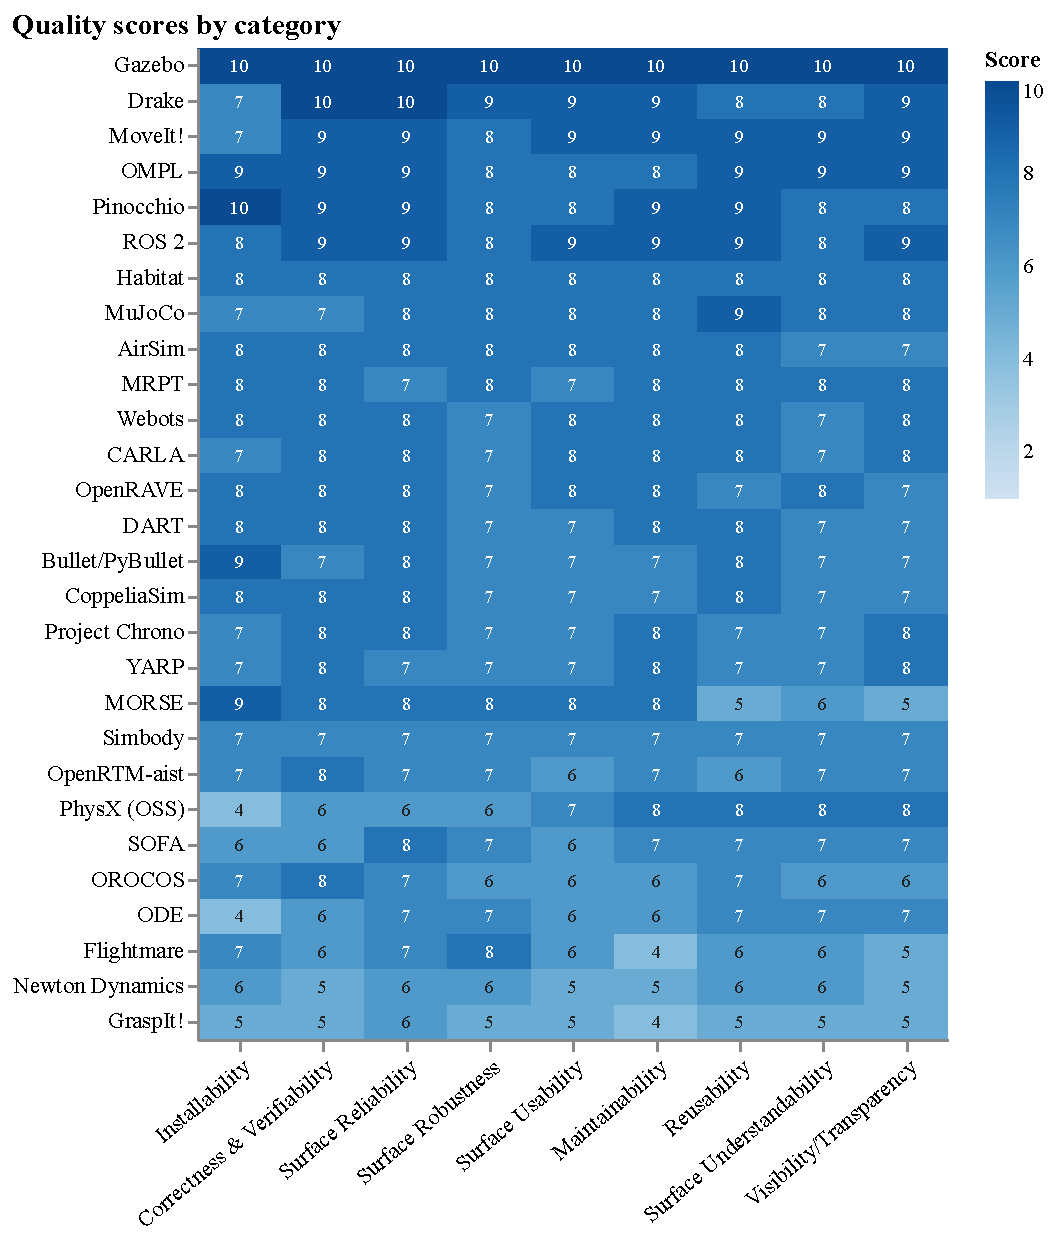
\includegraphics[width=0.95\textwidth]{figures/fig_quality_heatmap}
    \caption{Heatmap of the quality impression scores (1--10) for the 28 packages across the nine quality categories, ordered by unweighted mean.}
    \label{fig:quality-heatmap}
\end{figure}

\begin{figure}[htbp]
    \centering
    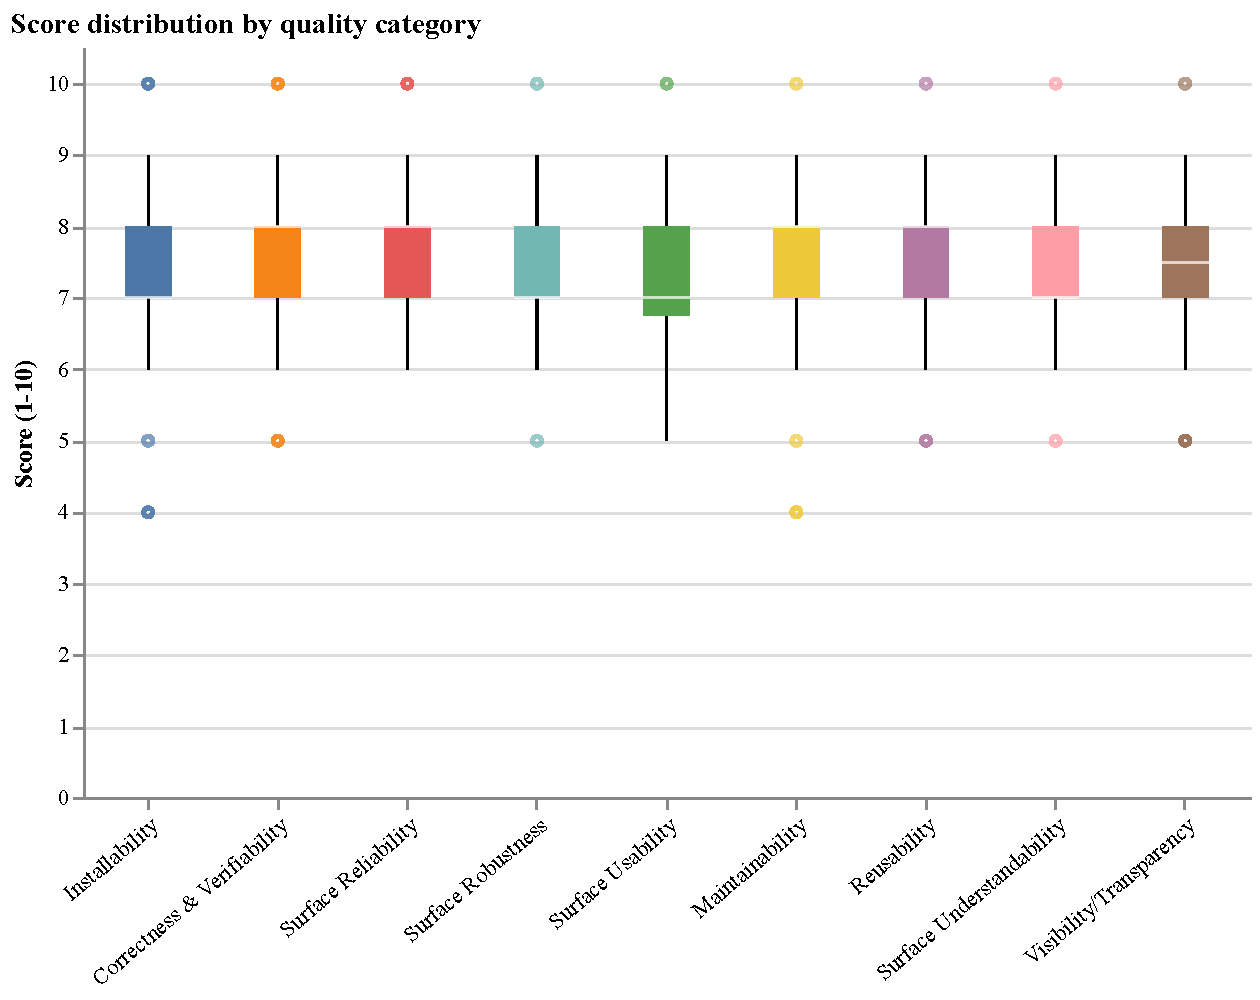
\includegraphics[width=0.95\textwidth]{figures/fig_category_distribution}
    \caption{Distribution of the impression scores across the 28 packages within each of the nine quality categories (box plots).}
    \label{fig:category-distribution}
\end{figure}

A handful of packages anchor the top of the table. Gazebo scores 10 in all nine categories, the only such sweep in the study. Within this template and time budget, no measured indicator separated it from the top of each scale; this is not a claim that the software is flawless. Drake and MoveIt! score 9 or 10 across most categories, and ROS~2, OMPL, and Pinocchio sit just below them. These packages share several traits: established stewardship (large organizations or active research groups), continuous contributor activity, comprehensive documentation, automated testing wired into CI/CD, and published contribution guidelines and release notes. None of these traits is individually decisive, but the combination separates the top tier from the rest.

For comparability with the descriptive summaries reported in the LBM and Medical Imaging assessments~\citep{Smith2024LBM,Smith2024MI}, Table~\ref{tab:overall-impressions} was also examined using a top-two coverage rule. A package was counted when it occupied one of the two highest distinct impression-score tiers in at least two of the nine quality categories. Six of the 28 packages (21\%) meet this criterion: Gazebo, Drake, MoveIt!, OMPL, Pinocchio, and ROS~2. The corresponding studies reported 67\% for LBM and almost 70\% for Medical Imaging. This difference does not establish that the MPS domain is unhealthy: the statistic is sensitive to tied scores, score calibration, the qualities measured, and the package-selection process in each study. Here it is used only to characterize the concentration of top-tier performance, which is clustered in a small leading group rather than broadly distributed across the sample.

\begin{figure}[htbp]
    \centering
    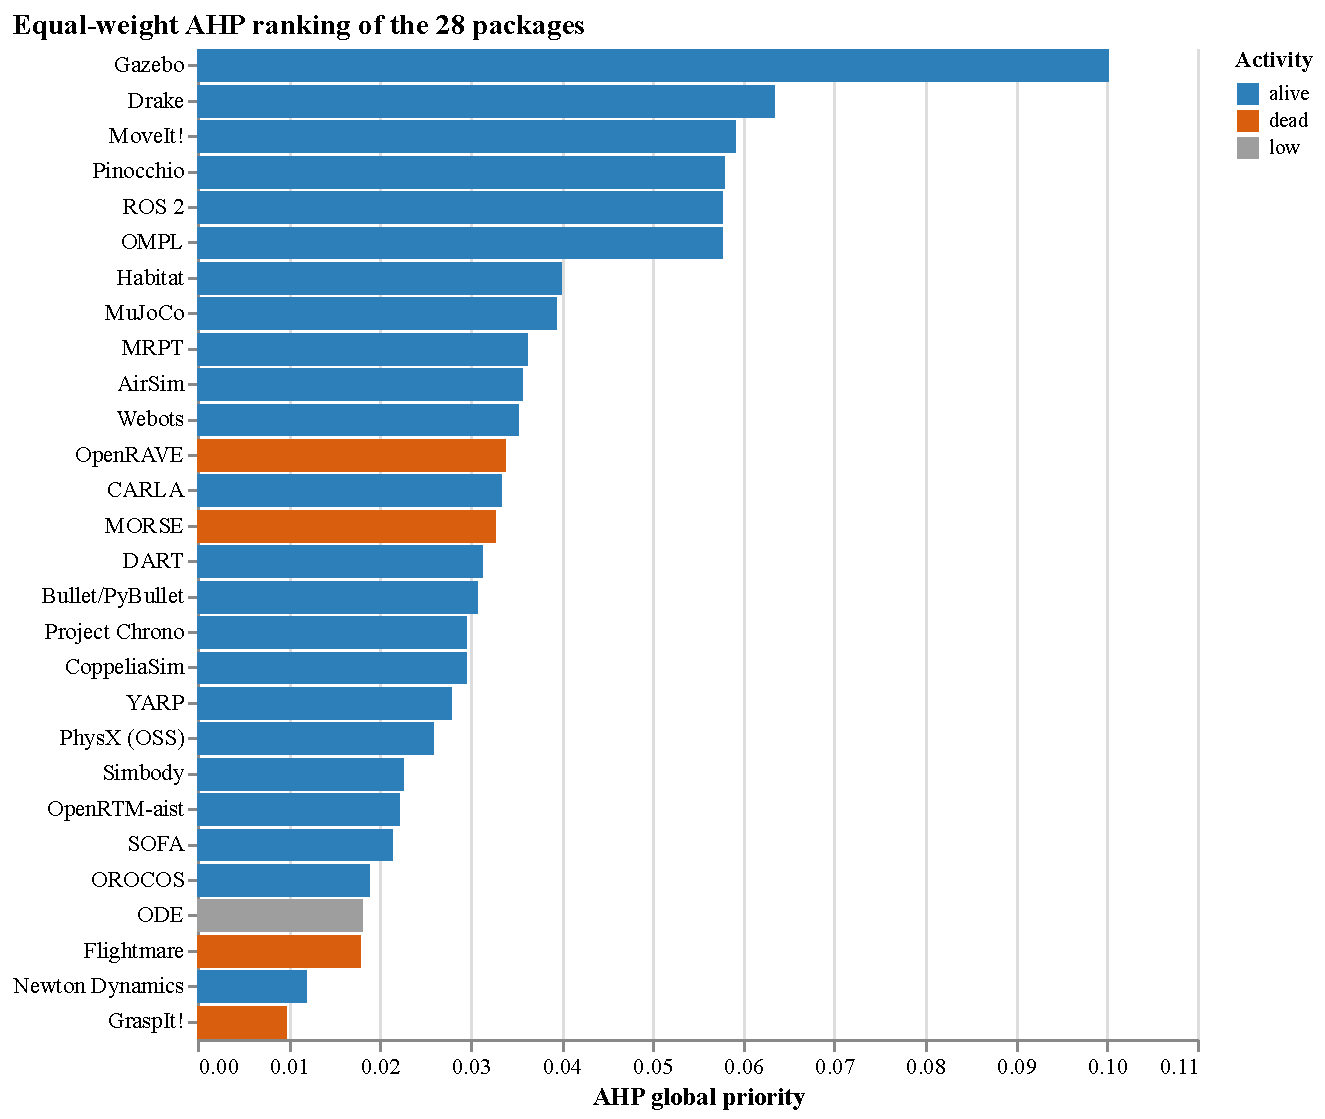
\includegraphics[width=0.92\textwidth]{figures/fig_ahp_ranking}
    \caption{Equal-weight AHP global-priority ranking ($c_k = 1/9$) of the 28 packages.}
    \label{fig:ahp-ranking}
\end{figure}

The AHP and arithmetic-mean orderings are close but not identical. Across the 28 packages, their ranks have Spearman correlation $\rho=0.987$ and Kendall correlation $\tau=0.944$. Gazebo, Drake, and MoveIt! occupy the same first three positions. The largest change is MORSE, which moves from 19th by arithmetic mean to 14th by AHP; all other packages move by at most three positions. AHP first converts each quality's pairwise score differences into a local priority vector and then aggregates those vectors. Equal criterion weights therefore do not reduce the calculation to an arithmetic mean of the original 1--10 scores.

To check that this ordering does not hinge on the precise impression scores, the AHP ranking was recomputed under a Monte~Carlo perturbation of its inputs. Each of the 252 score entries in Table~\ref{tab:overall-impressions} was independently scaled by a factor drawn uniformly from $[0.9, 1.1]$ (a $\pm 10\%$ perturbation clipped to the 1--10 range), and the equal-weight global priorities were re-derived over $1{,}000$ trials with a fixed random seed.

The ordering is well preserved: the mean Spearman rank correlation with the baseline is $0.97$ (minimum $0.87$) and the mean Kendall~$\tau$ is $0.88$ (minimum $0.74$). Gazebo remains top-ranked in every trial, and the two lowest, Newton~Dynamics and GraspIt!, are likewise fixed. The five highest-scoring packages after Gazebo never leave the top eight positions, though they are interchangeable within that band, with Drake alone ranging over ranks 2--6 (Figure~\ref{fig:ahp-sensitivity}).

The exact ordering among the leaders should therefore not be over-interpreted: the precise top-three and top-five sets recur in only $22\%$ and $26\%$ of trials, because their score gaps are smaller than the perturbation. The largest movement, up to ten positions, occurs in the densely packed middle of the table. The check thus supports the coarse structure of the ranking: a clear leader, a stable leading tier, a closely packed middle, and a fixed bottom (Section~\ref{sec:ahp-background}).

\begin{figure}[htbp]
    \centering
    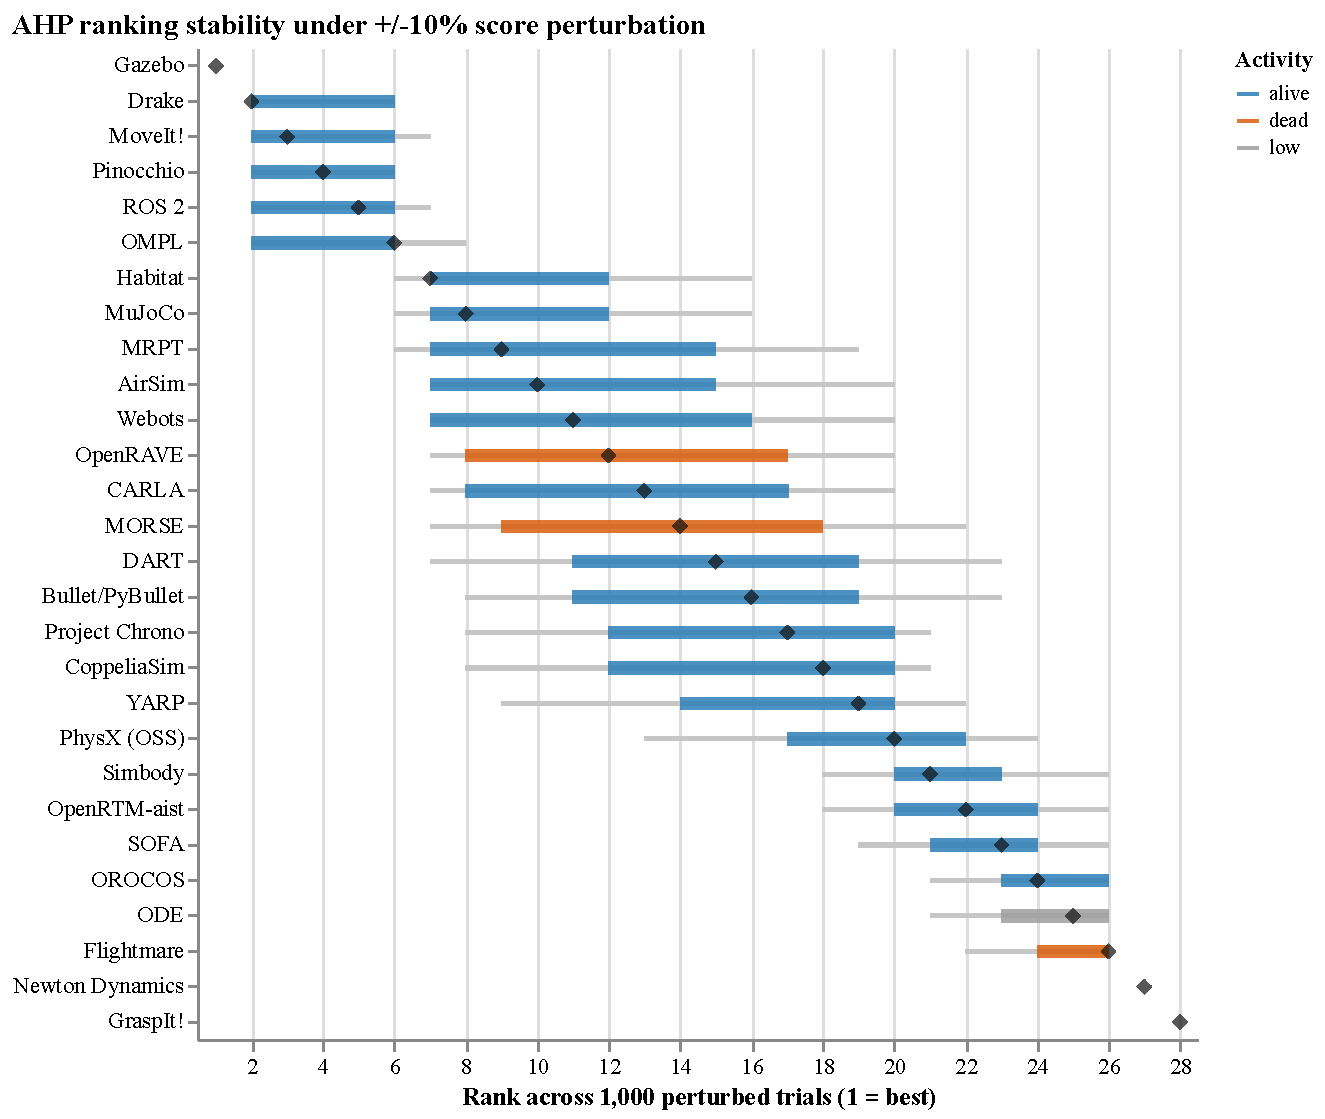
\includegraphics[width=0.92\textwidth]{figures/fig_ahp_sensitivity}
    \caption{Stability of the equal-weight AHP ranking under a $\pm 10\%$ score perturbation. Diamond, baseline rank; thick bar, 5th--95th percentile; thin line, full range.}
    \label{fig:ahp-sensitivity}
\end{figure}

The bottom of the table tracks maintenance status, but only loosely. GraspIt!, Flightmare, and MORSE (the dead packages of Section~\ref{sec:repository-project-metadata}) appear in the lower tier for most quality categories. Newton Dynamics, though technically alive at the May 2026 measurement date, joins them, reflecting its largely individual-maintained codebase and thin documentation infrastructure. OpenRAVE is also classified as dead under the 18-month rule, but its quality scores cluster in the middle of the table rather than the bottom; the documentation, test infrastructure, and codebase organization built during years of active development have not visibly degraded. In short, packages that go inactive tend to accumulate outdated documentation, broken installation procedures, and unresolved issues, but the rate at which they do so depends on the engineering capital accumulated before they went quiet.

Installability is generally strong across the MPS domain, most plausibly because of the widespread adoption of standard package managers (APT, pip, Conda), containerization (Docker), and CMake-based builds in the robotics community.

Documentation is universally present but varies in depth. All packages provide tutorials, user manuals, and API documentation, but the two indicators that record explicit engineering intent, coding standards and documented user characteristics, are far less common. The same gaps appear in the medical imaging and LBM samples~\citep{Smith2024MI,Smith2024LBM}, so they look more like patterns of research software practice than peculiarities of MPS. Figure~\ref{fig:key-indicators} summarizes this contrast across the template: the indicators tied to day-to-day installation and use sit at or near full coverage, while coding standards and documented user characteristics fall to 50\% and 4\%.

\begin{figure}[htbp]
    \centering
    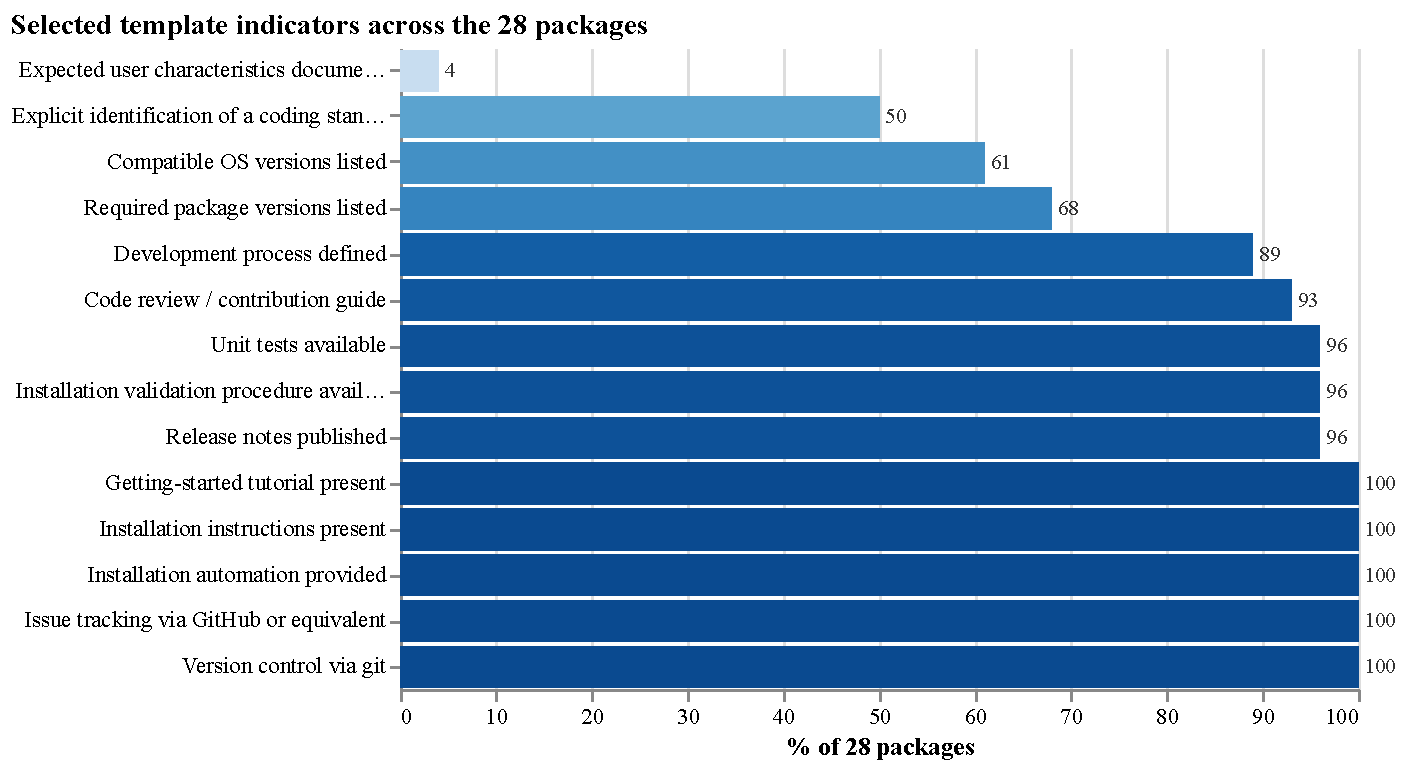
\includegraphics[width=0.92\textwidth]{figures/fig_key_indicators}
    \caption{Coverage of selected measurement-template indicators across the 28 packages, sorted from least to most common.}
    \label{fig:key-indicators}
\end{figure}

Repository activity is concentrated in a small subset of packages, with a few large or long-running projects accounting for a disproportionate share of total commits while several others show minimal activity in the last 12 months (Section~\ref{sec:repository-metrics-results}).
\section{Comparison with Community Indicators}
\label{sec:quality-vs-community}

The AHP priority (Section~\ref{sec:overall-observations}) combines the nine measured quality scores, while repository stars capture attention accumulated by a particular GitHub repository. Table~\ref{tab:quality-vs-community} compares these two rankings; ODE is omitted from the star ranking because its Bitbucket watcher count is not the same measure.

\begin{table}[p]
\centering
\caption{Equal-weight AHP rank versus GitHub stars rank. $\Delta = S - A$: positive values indicate a higher AHP rank than stars rank; negative values indicate a higher stars rank. Ties receive the same rank. ODE is excluded from the stars rank because its host reports watchers rather than GitHub stars (Table~\ref{tab:repository-metrics}).}
\label{tab:quality-vs-community}
\small
\singlespacing
\begin{tabular}{@{}P{2.5cm}rcrrr@{}}
\toprule
\textbf{Software} & \textbf{AHP Priority} & \textbf{A-Rank} & \textbf{Stars} & \textbf{S-Rank} & \textbf{$\Delta$} \\
\midrule
Gazebo          & 0.10012 & 1  & 1,337  & 17 & $+16$ \\
Drake           & 0.06339 & 2  & 4,025  & 8  & $+6$  \\
MoveIt!         & 0.05909 & 3  & 1,803  & 15 & $+12$ \\
Pinocchio       & 0.05795 & 4  & 3,354  & 10 & $+6$  \\
ROS~2           & 0.05775 & 5  & 5,475  & 5  & $0$   \\
OMPL            & 0.05765 & 6  & 2,047  & 14 & $+8$  \\
Habitat         & 0.03994 & 7  & 3,662  & 9  & $+2$  \\
MuJoCo          & 0.03939 & 8  & 13,440 & 4  & $-4$  \\
MRPT            & 0.03621 & 9  & 2,133  & 13 & $+4$  \\
AirSim          & 0.03571 & 10 & 18,159 & 1  & $-9$  \\
Webots          & 0.03527 & 11 & 4,345  & 7  & $-4$  \\
OpenRAVE        & 0.03387 & 12 & 801    & 21 & $+9$  \\
CARLA           & 0.03336 & 13 & 13,941 & 3  & $-10$ \\
MORSE           & 0.03276 & 14 & 367    & 23 & $+9$  \\
DART            & 0.03128 & 15 & 1,081  & 19 & $+4$  \\
Bullet/\allowbreak{}PyBullet & 0.03078 & 16 & 14,465 & 2 & $-14$ \\
Project Chrono  & 0.02953 & 17 & 2,836  & 11 & $-6$  \\
CoppeliaSim     & 0.02953 & 17 & 146    & 25 & $+8$  \\
YARP            & 0.02785 & 19 & 590    & 22 & $+3$  \\
PhysX (OSS)     & 0.02586 & 20 & 4,532  & 6  & $-14$ \\
Simbody         & 0.02257 & 21 & 2,521  & 12 & $-9$  \\
OpenRTM-aist    & 0.02216 & 22 & 24     & 26 & $+4$  \\
SOFA            & 0.02138 & 23 & 1,194  & 18 & $-5$  \\
OROCOS          & 0.01893 & 24 & 879    & 20 & $-4$  \\
ODE             & 0.01810 & 25 & ---    & ---& ---   \\
Flightmare      & 0.01793 & 26 & 1,353  & 16 & $-10$ \\
Newton Dynamics& 0.01195 & 27 & 24     & 26 & $-1$  \\
GraspIt!        & 0.00971 & 28 & 213    & 24 & $-4$  \\
\bottomrule
\end{tabular}
\end{table}

The 28 packages fall into four broad patterns in Table~\ref{tab:quality-vs-community}.

\textbf{Rough agreement at the top.} ROS~2 has rank 5 on both indicators. Drake ($\Delta=+6$), Pinocchio ($+6$), and Habitat ($+2$) also sit near the top of both lists.

\textbf{High AHP priority, lower repository visibility.} Gazebo ($\Delta=+16$), MoveIt! ($+12$), and OMPL ($+8$) are near the top of the AHP ranking but lower in stars. Gazebo's current repository omits attention accumulated before its repository reorganization; OMPL and MoveIt! are also used as dependencies inside larger workflows.

\textbf{High repository visibility, mid-pack AHP priority.} Bullet/PyBullet and PhysX (both $\Delta=-14$), CARLA ($-10$), and AirSim ($-9$) sit near the top in stars but in the middle or lower half of the AHP ranking. Their audiences extend into gaming, autonomous-driving research, and real-time physics, so repository attention need not track the research-software practices measured here.

\textbf{Low on both indicators.} GraspIt! ($\Delta=-4$) and Newton Dynamics ($-1$) are near the bottom on both lists. Newton Dynamics is a repository-migration case (Section~\ref{sec:repository-project-metadata}); its original repository would place it higher in stars without changing its AHP result.

These patterns agree with the medical imaging study's finding that repository popularity and measurement-based rankings do not have a simple relationship~\citep{Smith2024MI}. The comparison is descriptive: stars are host-, age-, and migration-dependent, so Table~\ref{tab:quality-vs-community} does not test whether engineering practice causes popularity (Section~\ref{sec:threat-construct-validity}).
